
\paragraph{Goal}
There are many programming languages, and many \acrlongpl{IDE}.
Traditionally, every \acrshort{IDE} would have a special integration for every language it supported.
Extracting tokens, keywords, providing auto completion, code formatting and so on.
This leads to a lot of rework every time a new \acrshort{IDE} comes around, and duplication of work every time a new programming language is supported.
Essentially, every $m$ number of \acrshortpl{IDE} that support an $n$ number of programming languages result in $m\times{}n$ different integrations.
This is illustrated in the left side of \cref{fig:lsp-m-times-n}.\\

A solution to this $m\times{}n$ problem is the \textit{\acrlong{LSP}} (\acrshort{LSP}).
If instead, every \acrshort{IDE} has a generic text editor for all languages, they only need to support the \acrshort{LSP}.
Once an editor ``talks'' \acrshort{LSP}, it can support \textbf{all programming languages} that have a \acrshort{LSP} \textit{language server}.
Likewise, a programming language only needs to develop \textbf{one language server}, and it supports all \acrshortpl{IDE} that use \acrshort{LSP}~\cite{microsoftOverview}.
This is shown in the right side of \cref{fig:lsp-m-times-n}.\\

This protocol was created by Microsoft, and is in use today on \gls{VSCode}.
Many \acrshortpl{IDE} and text editors have adopted it afterwards, like \gls{Eclipse} (with LSP4E), Atom, Vim, Sublime Text, Spyder and more, via both official and unofficial plugins to these \acrshortpl{IDE}~\cite{microsoftToolsSupportingLSP}.
The protocol is quite extensive, and defines approximately 40 different requests with corresponding responses, 20 notification types, in addition to data structures needed to support all of these~\cite{microsoftLanguageServerProtocol2021}.

\begin{figure}[htbp]  % order of priority: h here, t top, b bottom, p page
  \centering
  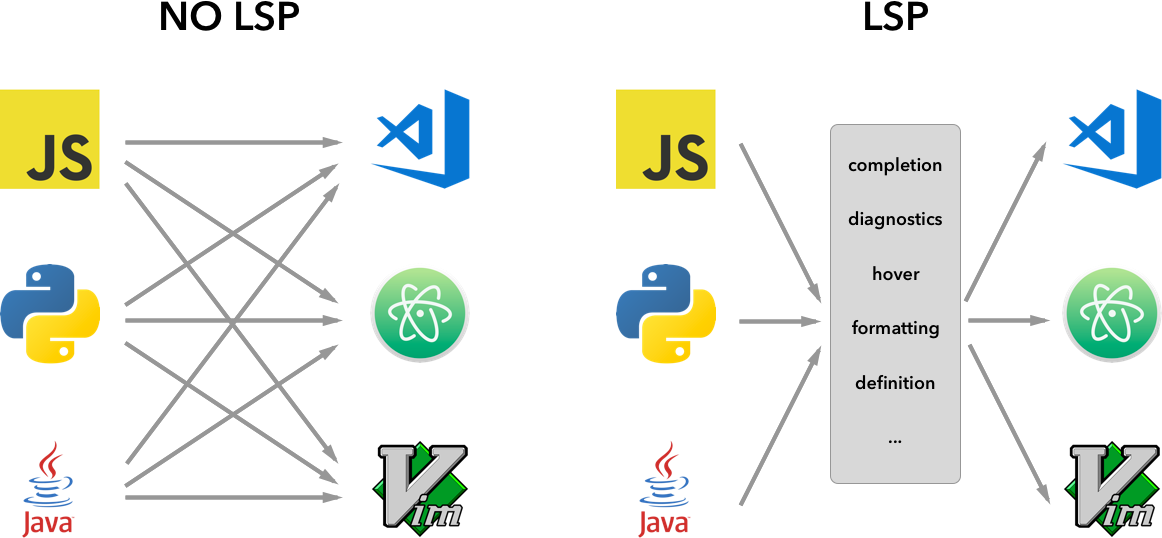
\includegraphics[width=\textwidth]{figures/pre-project/lsp-languages-editors.png}
  \caption[The Language Server Protocol Benefits]{The benefits of using the \acrshort{LSP}. The left side shows all the integrations (as arrows) required for 3 languages (javascript, python, java) and 3 editors (VSCode, Atom, Vim), without the \acrshort{LSP}.
  The right side shows how the \acrshort{LSP} can reduce the amount of work by unifying the common elements of programming language editors into a standard protocol. Figure copied from~\textcite{microsoftLanguageServerExtension2020}.}\label{fig:lsp-m-times-n}
\end{figure}

\paragraph{Protocol}
The \acrlong{LSP} is based on a \textit{Base Protocol}.
This Base Protocol is similar to HTTP, in that it has a \textit{header} section and a \textit{content} section.
The content section contains \acrfullpl{RPC}, using a protocol called \gls{JSON-RPC}.
This is shown in \cref{fig:lsp-architecture}.

\begin{figure}[htbp]  % order of priority: h here, t top, b bottom, p page
  \centering
  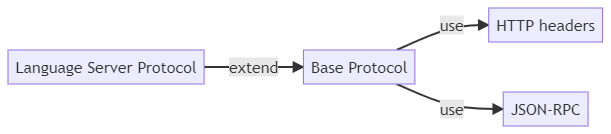
\includegraphics[width=\textwidth]{figures/pre-project/lsp-protocol.png}
  \caption[LSP Protocol Design]{The \acrlong{LSP} protocol extends a Base Protocol with JSON-RPC content.}\label{fig:lsp-architecture}
\end{figure}

\subsection{Base Protocol}\label{sec:base-protocol}

All communication in \acrshort{LSP} uses concepts from the Base Protocol.
This protocol has a header and content section, as mentioned above.
Conceptually, the protocol assumes there is one \textit{client} and one \textit{server} which communicates.
Note that the server can also initiate requests to the client.
In addition, the Base Protocol defines specific types of messages: \textit{Request Message}, \textit{Response Message}, \textit{Notification Message}, and \textit{\$ Notifications and Requests}~\cite{microsoftLanguageServerProtocol2021}.

\paragraph{Header}
The header is comparable to a HTTP header, with key-value pairs separated by colon, and a line break for each new pair.
The currently supported header keys are \texttt{Content-Length} and \texttt{Content-Type}.
The \texttt{Content-Length} specifies how many bytes the content is~\cite{microsoftLanguageServerProtocol2021}.

\paragraph{Content}
The content section contains the actual message data, like requests and responses.
This section follows the \gls{JSON-RPC} protocol, described later in \cref{sec:json-rpc}~\cite{microsoftLanguageServerProtocol2021}.

\paragraph{Request and Response}
A Request Message describes a request from a client to the server.
This must have an ID, a method name (for \gls{RPC}) and parameter values for the method.
When a client sends a Request, it means that the server should execute the given method with the given parameters.
The server must then respond with the results of the execution in a Response Message.
This Response must have the id of the originating Request, as well as the results or an error~\cite{microsoftLanguageServerProtocol2021}.\\

An example of a Request is shown in \cref{lst:lsp-example}.
It is the \texttt{textDocument/signatureHelp} method, specifying a \texttt{textDocument} and \texttt{position} with parameter values for the \texttt{textDocument/signatureHelp} method call.

\begin{lstlisting}[caption={A Request Message Example}, label={lst:lsp-example}]
Content-Length: 201

{
    "jsonrpc":"2.0",
    "id":"1",
    "method":"textDocument/signatureHelp",
    "params": {
        "textDocument": { "uri": "file:/..." },
        "position": { "line": 5, "character": 3 },
    }
}
\end{lstlisting}


\paragraph{Notification}
A Notification Message is more like an event.
It does not have an ID, and does not get a Response Message in return.
The Notification, like the Request, specifies a method and parameter values~\cite{microsoftLanguageServerProtocol2021}.

\paragraph{\$ Notifications and Requests}
If a Notification or Request has a \lstinline{$/} at the start of the method name, it is an optional and protocol implementation-specific message.
Not all clients and servers handle these messages.
A notification can be ignored, and a request must be answered with a specific error, if the message is not implemented.

\subsection{Language Server Protocol}
The \acrfull{LSP} defines \gls{JSON-RPC} requests, response and notification messages that are sent in the Base Protocol.
These are specified as method names and parameter values, as well as semantics and rules related to the sequences, responses to, and content of these messages.
\acrshort{LSP} also defines a set of \gls{JSON} data structures, which are used in the messages as parameter values and response types~\cite{microsoftLanguageServerProtocol2021}.
The protocol is versioned, where \texttt{3.16} is the current version.\\

The \acrshort{LSP} defines many messages, related to these categories: 
\begin{itemize}
  \item Window
  \item Telemetry
  \item Client
  \item Workspace
  \item Text Synchronization
  \item Diagnostics
  \item Language Features
\end{itemize}
The most important category is Language Features, which define Requests such as: completion, hover, signature help, references, code action, formatting, rename, and more.
The full list is available in the \citetitle{microsoftLanguageServerProtocol2021}~\cite{microsoftLanguageServerProtocol2021}.
